\documentclass{../../PublicResources/DocClass}

    \DocumentTitle{「切换语言」使用手册}
    \DocumentSubtitle{Blender插件}
    \DocumentCreatedDate{2020/6/5}

    \LinkBlogPost{https://mister-kin.github.io/manuals/toggle-language/}
    \LinkPDFSource{https://github.com/Mister-Kin/OpenDocs/tree/master/Manuals/ToggleLanguage}
    \LinkVideo{}

    \AuthorName{Mr. Kin}
    \AuthorEmail{im.misterkin@gmail.com}
    \AuthorBlog{https://mister-kin.github.io/}

\begin{document}
    \pagenumbering{Roman} % 大写罗马字母样式页码。
    \maketitle
    \addcontentsline{toc}{chapter}{封面}
    \frontmatter
    \phantomsection
\begin{center}
    {\bfseries\sffamily\Large 关于作者}
\end{center}
\addcontentsline{toc}{chapter}{关于作者}

\subsection*{\bfseries \sffamily 关于我}
\begin{wrapfigure}[3]{L}{60pt}
    \vspace*{-20pt}
    \centering
    
\includegraphics{kin-logo}
\end{wrapfigure}
\textbf{Mr. Kin},广东客家仁,程序猿,CG和游戏爱好者,一枚极客。翻译UP主,个人UP主。不定时在B站直播日常:码代码,码博客,翻译,做视频,做教程。 ($\vartheta$$\bullet$\_$\bullet$)$\vartheta$ \hyperlink{follow}{\emph{(点击关注我!)}}

\subsection*{\bfseries \sffamily 开源建设}

\noindent {\bfseries \sffamily 开源软件的中文化翻译}

\begin{itemize}
    \item \href{https://docs.krita.org/zh_CN/}{Krita手册}:2018.8.5 - \href{https://crowdin.com/profile}{2019.4.23}
    \item \href{https://docs.blender.org/manual/zh-hans/latest/}{Blender手册}:2019.7.20 - \href{https://www.blendercn.org/5812.html?tdsourcetag=s_pctim_aiomsg}{2019.9.4} - 至今(\href{https://developer.blender.org/p/Mr_Kin/}{翻译维护})
\end{itemize}

\subsection*{\bfseries \sffamily \hypertarget{contact}{联系方式}}
\vspace*{-1ex}
\noindent {\footnotesize \color{red} \em 注:联系时请注明身份,谢谢!}

\begin{itemize}
    \item QQ:\href{tencent://AddContact/?fromId=45&fromSubId=1&subcmd=all&uin=2312463626&website=www.oicqzone.com}{2312463626}\emph{\color{red}(点击号码加好友)}
    \item 邮箱:2312463626@qq.com ; im.misterkin@gmail.com
\end{itemize}

\subsection*{\bfseries \sffamily \hypertarget{follow}{关注渠道}}
\vspace*{-1ex}
\noindent {\footnotesize \color{red} \em 注:点击文字即可跳转关注!}
\vspace*{-2ex}

\begin{figure}[htbp]
    \centering
    
\includegraphics[scale=0.2]{WechatOfficialAccounts.png}
\end{figure}
\vspace*{-4ex}

\begin{figure}[htbp]
    \centering
    \begin{minipage}[t]{0.2\textwidth}
        \centering
        \caption*{\href{https://mister-kin.github.io}{博客 - Blog}}
        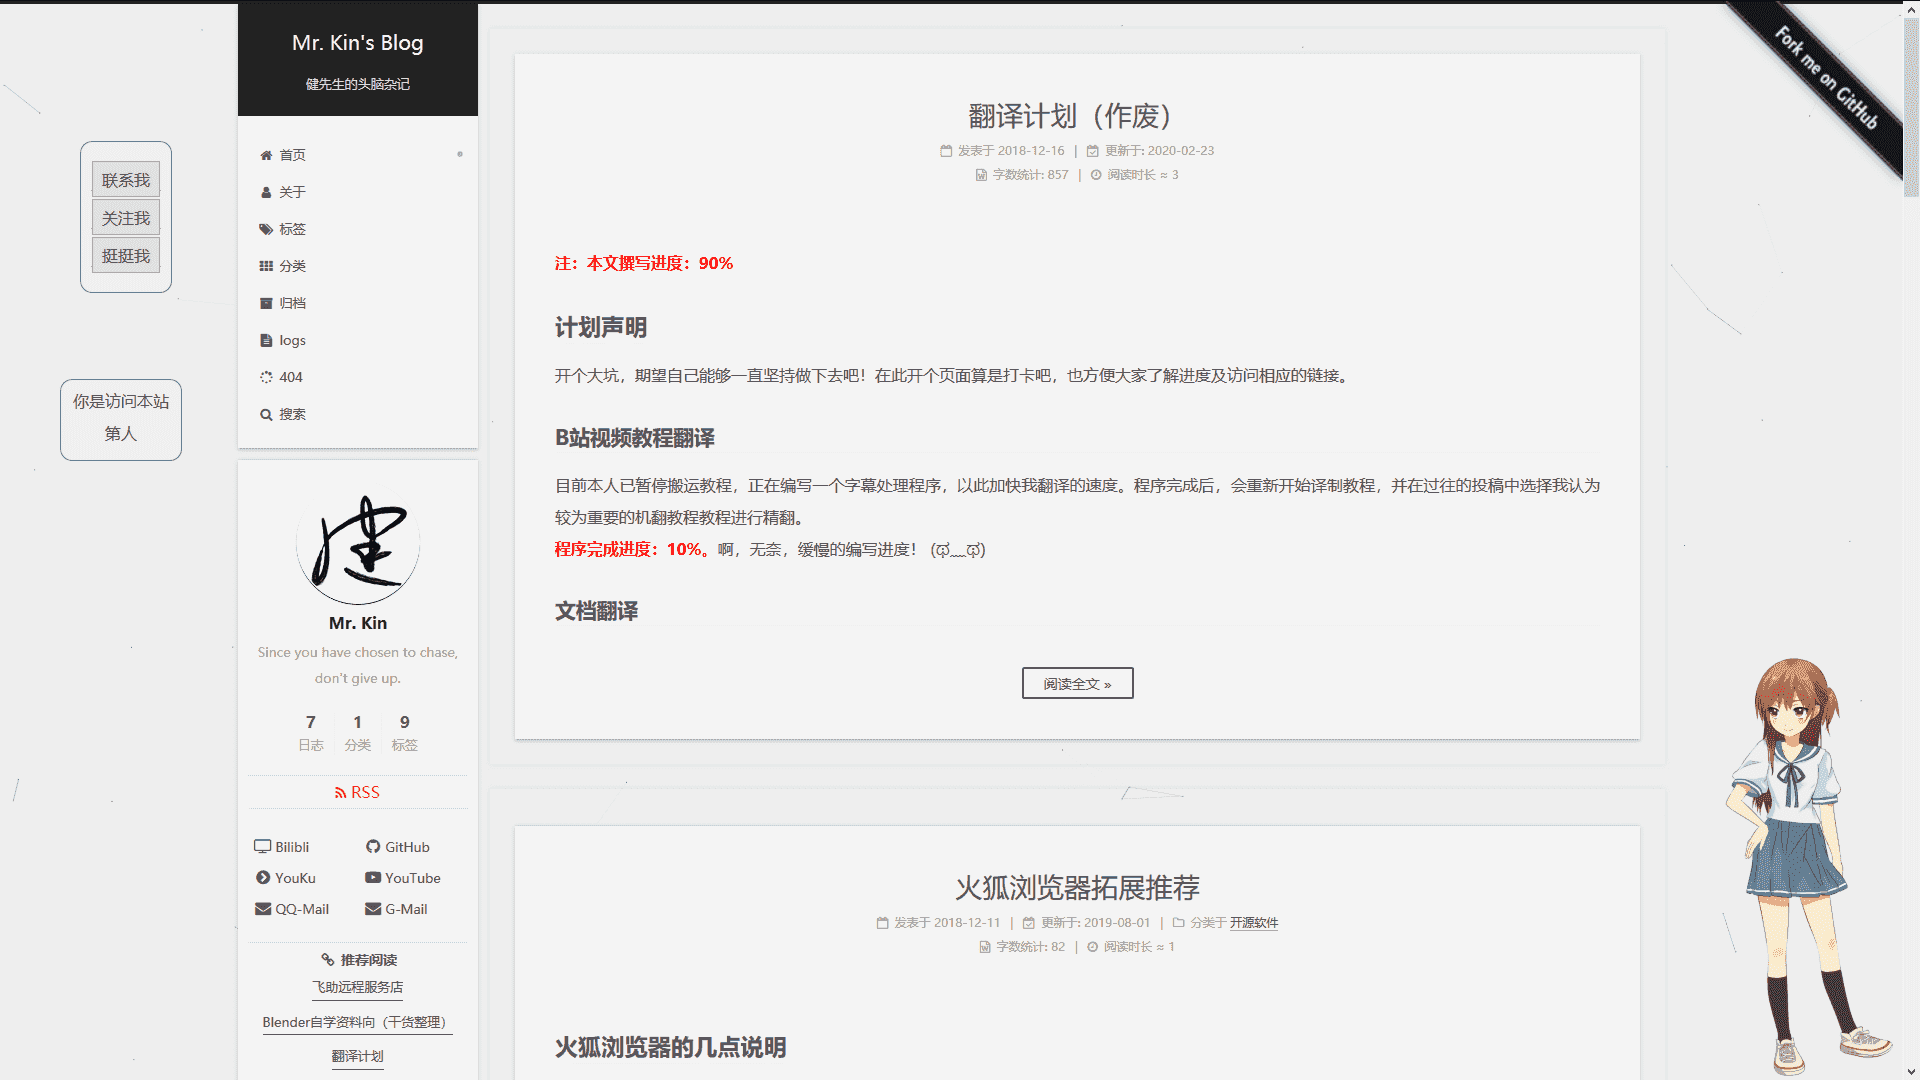
\includegraphics[scale=0.055]{Blog}
    \end{minipage}
    \qquad
    \begin{minipage}[t]{0.2\textwidth}
        \centering
        \caption*{\href{https://github.com/mister-kin}{Github}}
        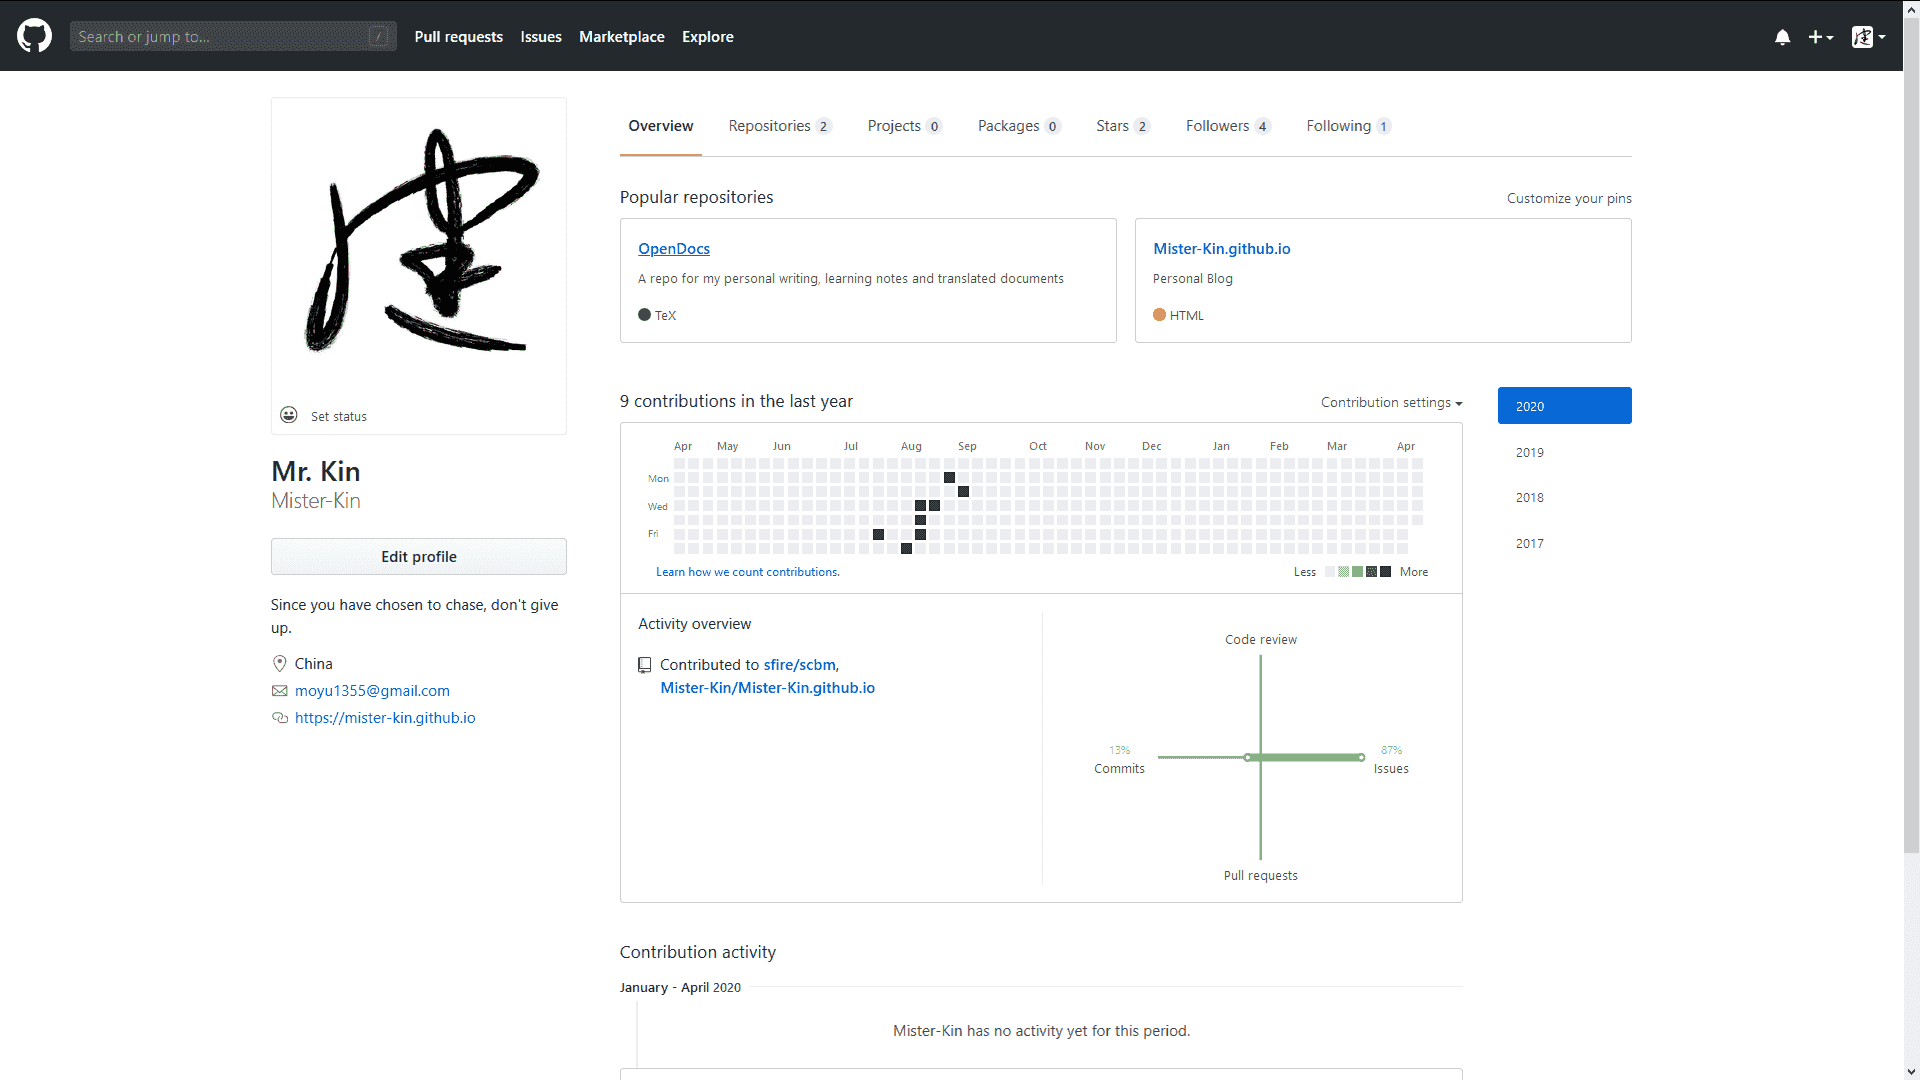
\includegraphics[scale=0.055]{Github}
    \end{minipage}
    \qquad
    \begin{minipage}[t]{0.2\textwidth}
        \centering
        \caption*{\href{https://weibo.com/6270111192/profile?topnav=1&wvr=6&is_all=1}{微博 - Weibo}}
        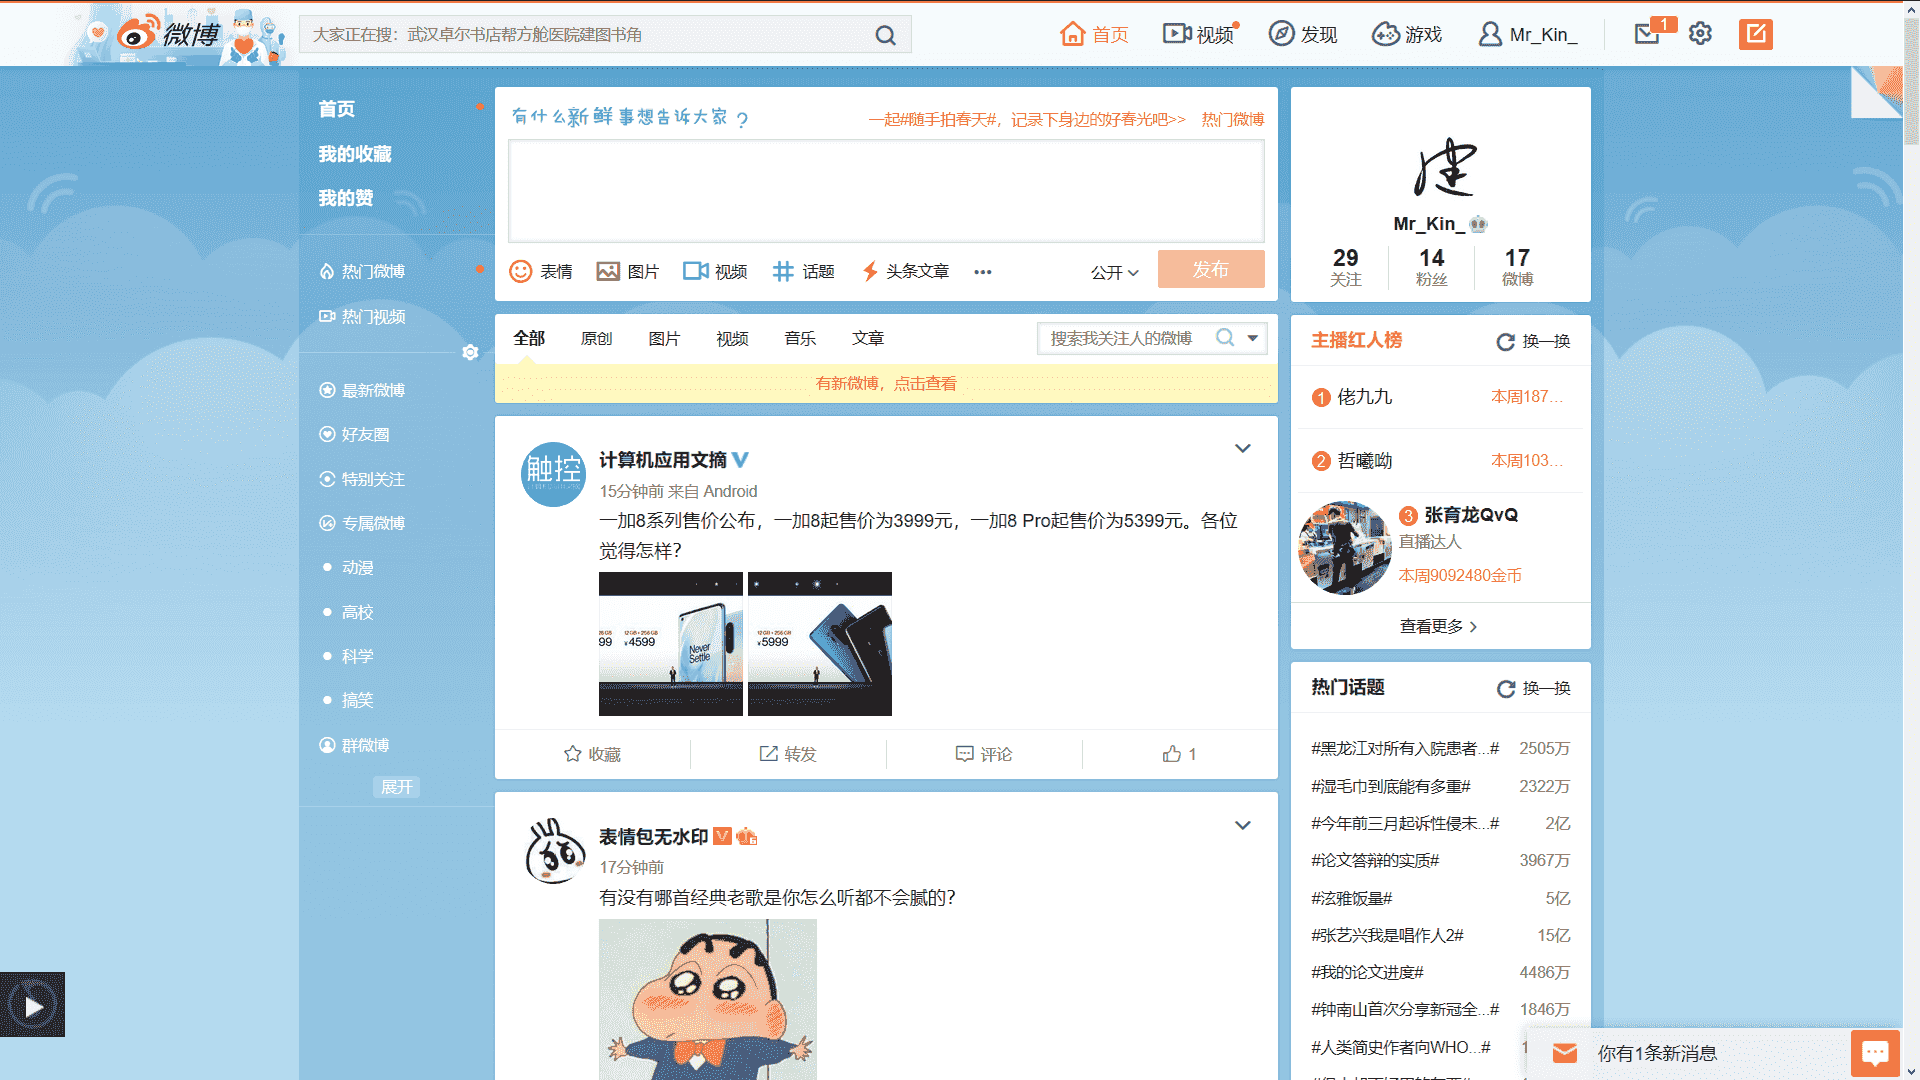
\includegraphics[scale=0.055]{Weibo}
    \end{minipage}
    \qquad
    \begin{minipage}[t]{0.2\textwidth}
        \centering
        \caption*{\href{https://www.zhihu.com/people/drwu-94}{知乎 - Zhihu}}
        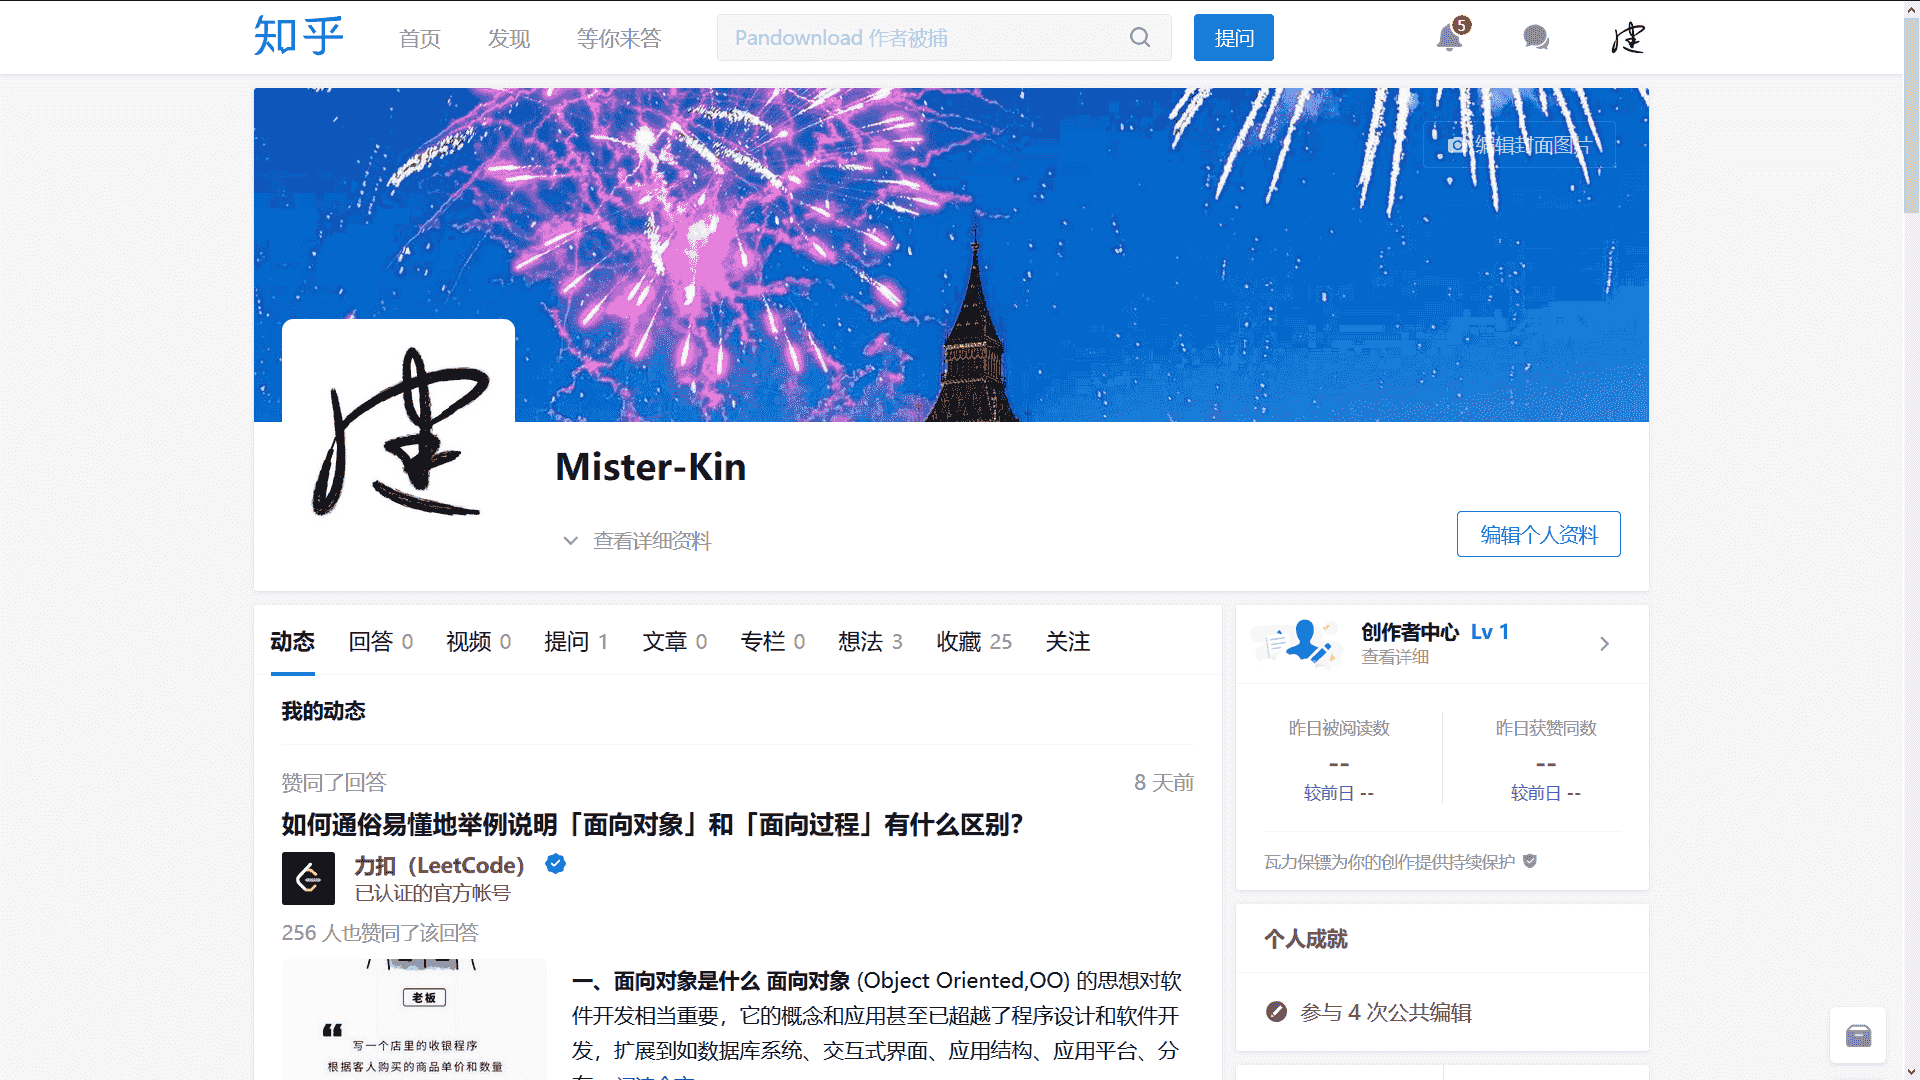
\includegraphics[scale=0.055]{Zhihu}
    \end{minipage}

    \vspace*{3ex}

    \begin{minipage}[t]{0.2\textwidth}
        \centering
        \caption*{\href{http://space.bilibili.com/17025250?}{B站 - Bilibili}}
        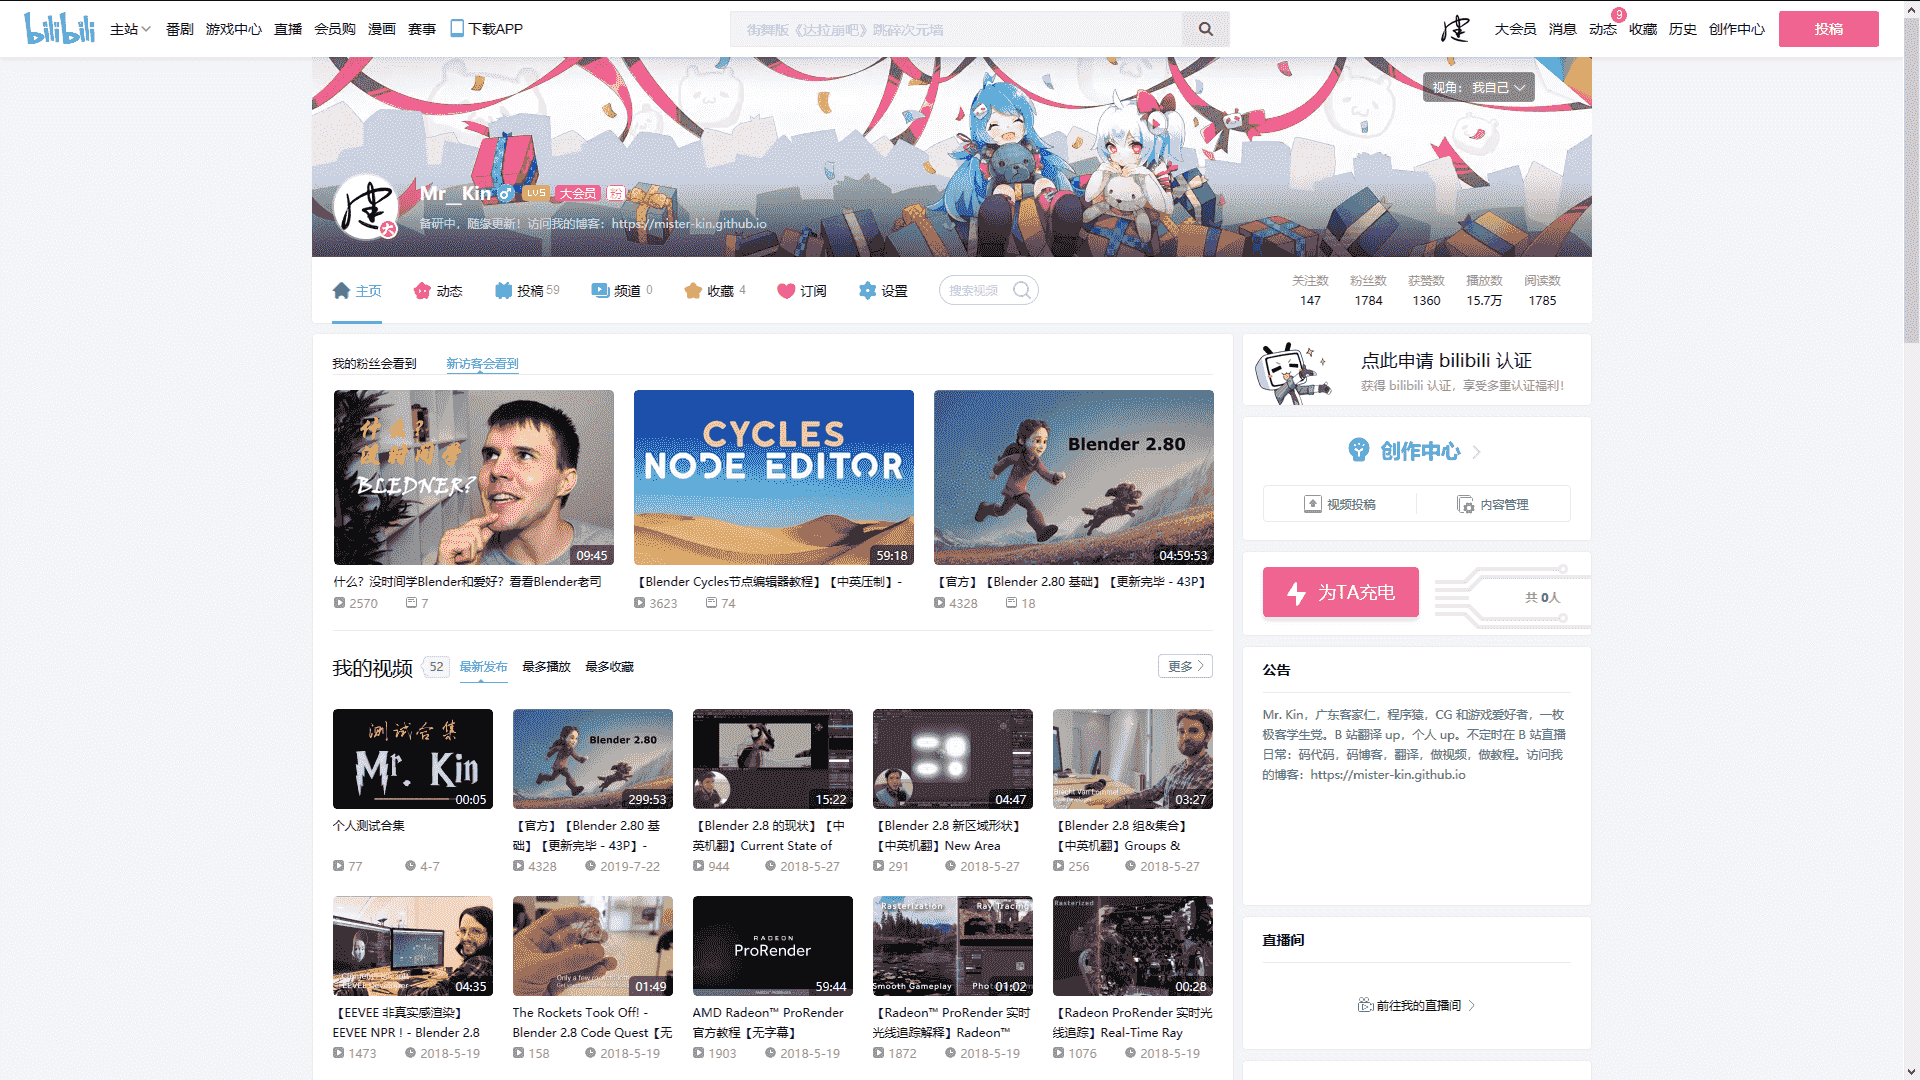
\includegraphics[scale=0.055]{Bilibili}
    \end{minipage}
    \qquad
    \begin{minipage}[t]{0.2\textwidth}
        \centering
        \caption*{\href{http://i.youku.com/i/UNjA3MTk5Mjgw?spm=a2hzp.8253869.0.0}{优酷 - Youku}}
        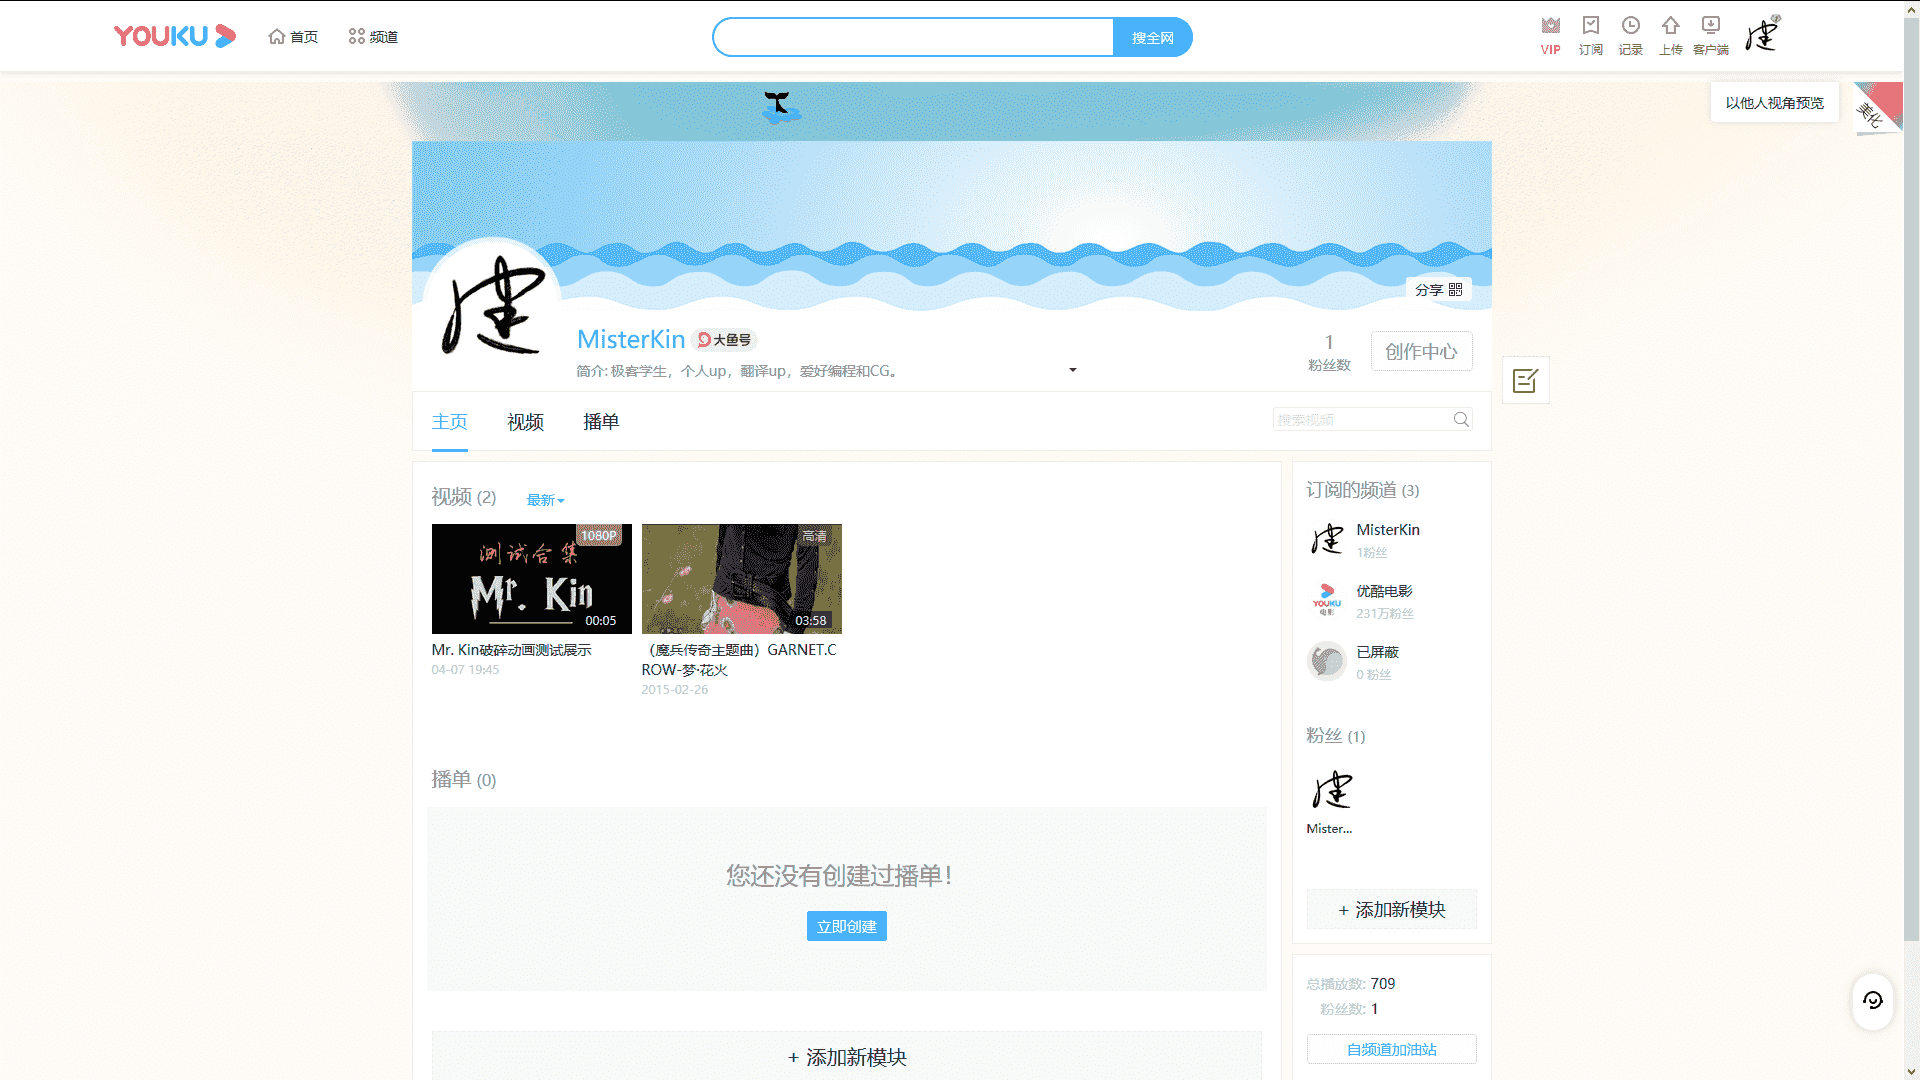
\includegraphics[scale=0.055]{Youku}
    \end{minipage}
    \qquad
    \begin{minipage}[t]{0.2\textwidth}
        \centering
        \caption*{\href{https://www.toutiao.com/c/user/835254071079053/\#mid=1663279303982091}{头条 - Headline}}
        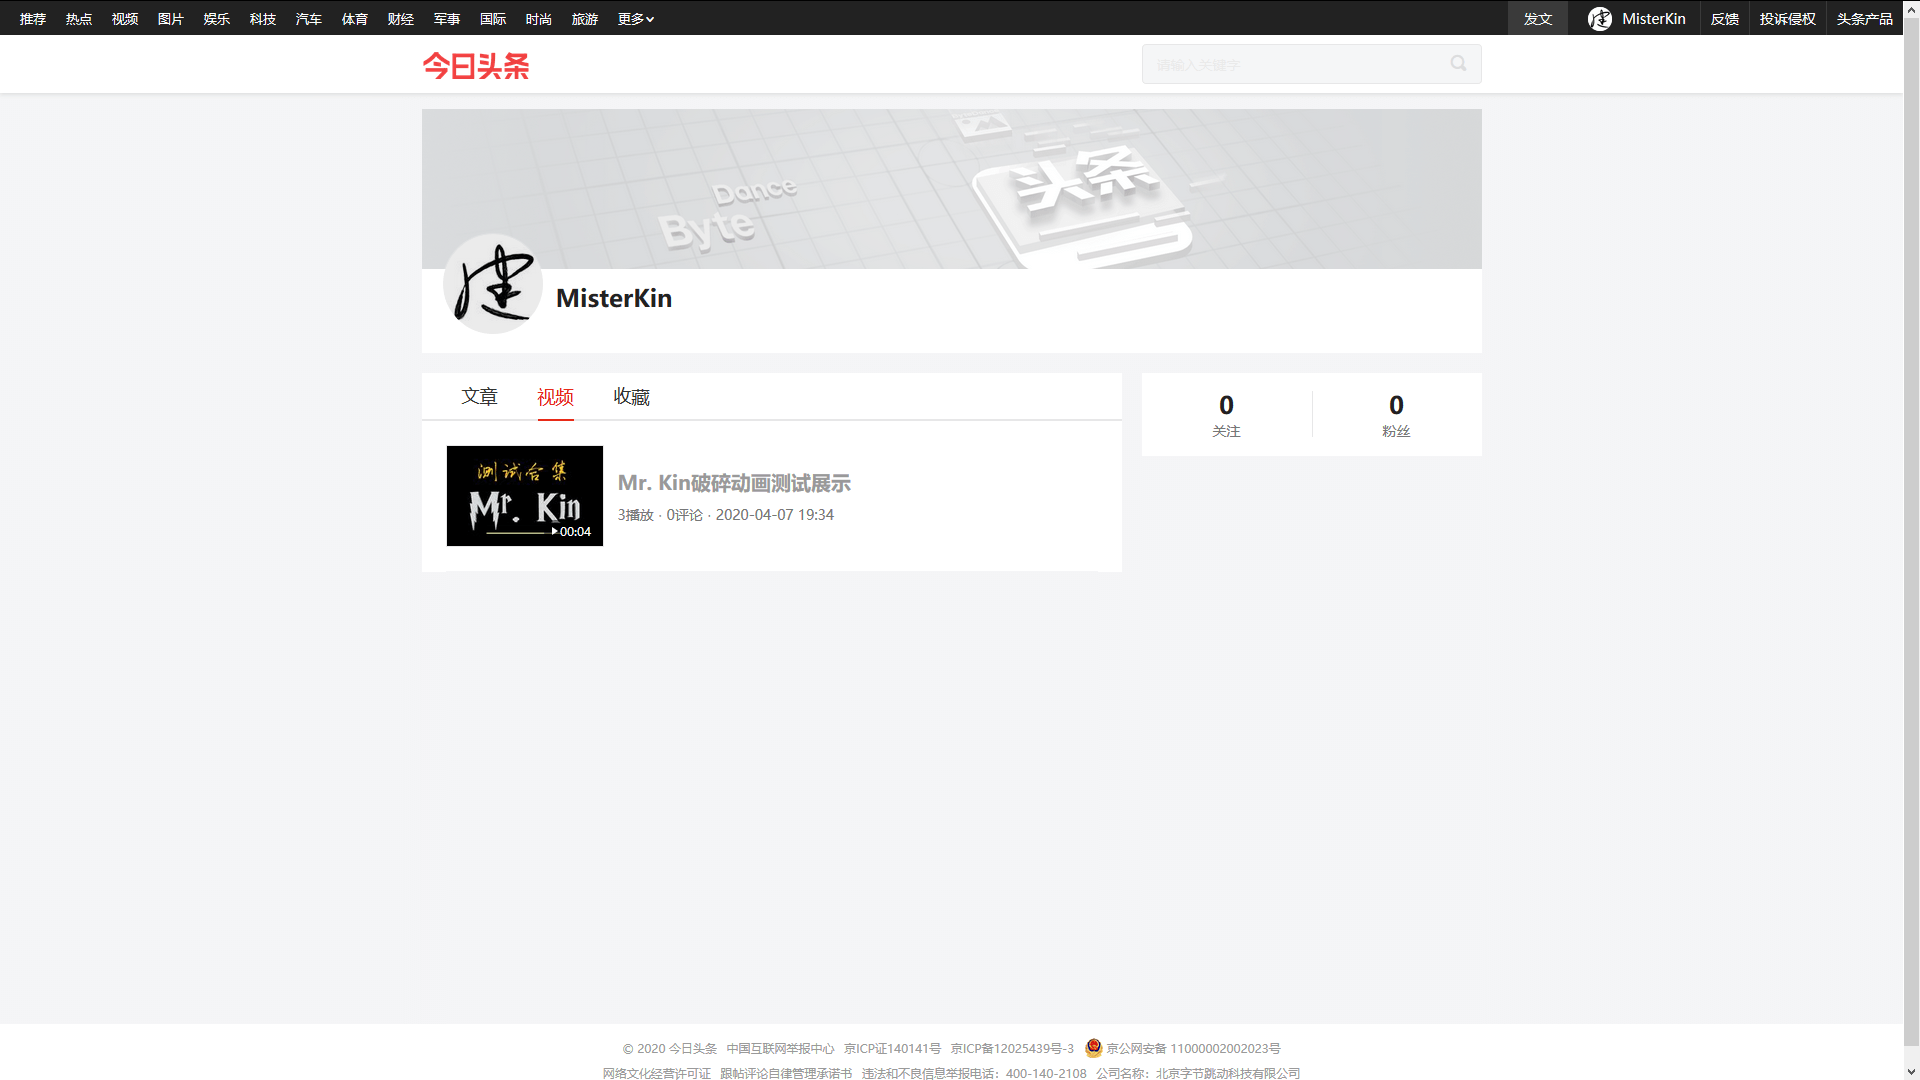
\includegraphics[scale=0.055]{Headline}
    \end{minipage}
    \qquad
    \begin{minipage}[t]{0.2\textwidth}
        \centering
        \caption*{\href{https://www.youtube.com/channel/UCXqjfWLzMlRKxGC8syWj17Q?view_as=public}{油管 - Youtube}}
        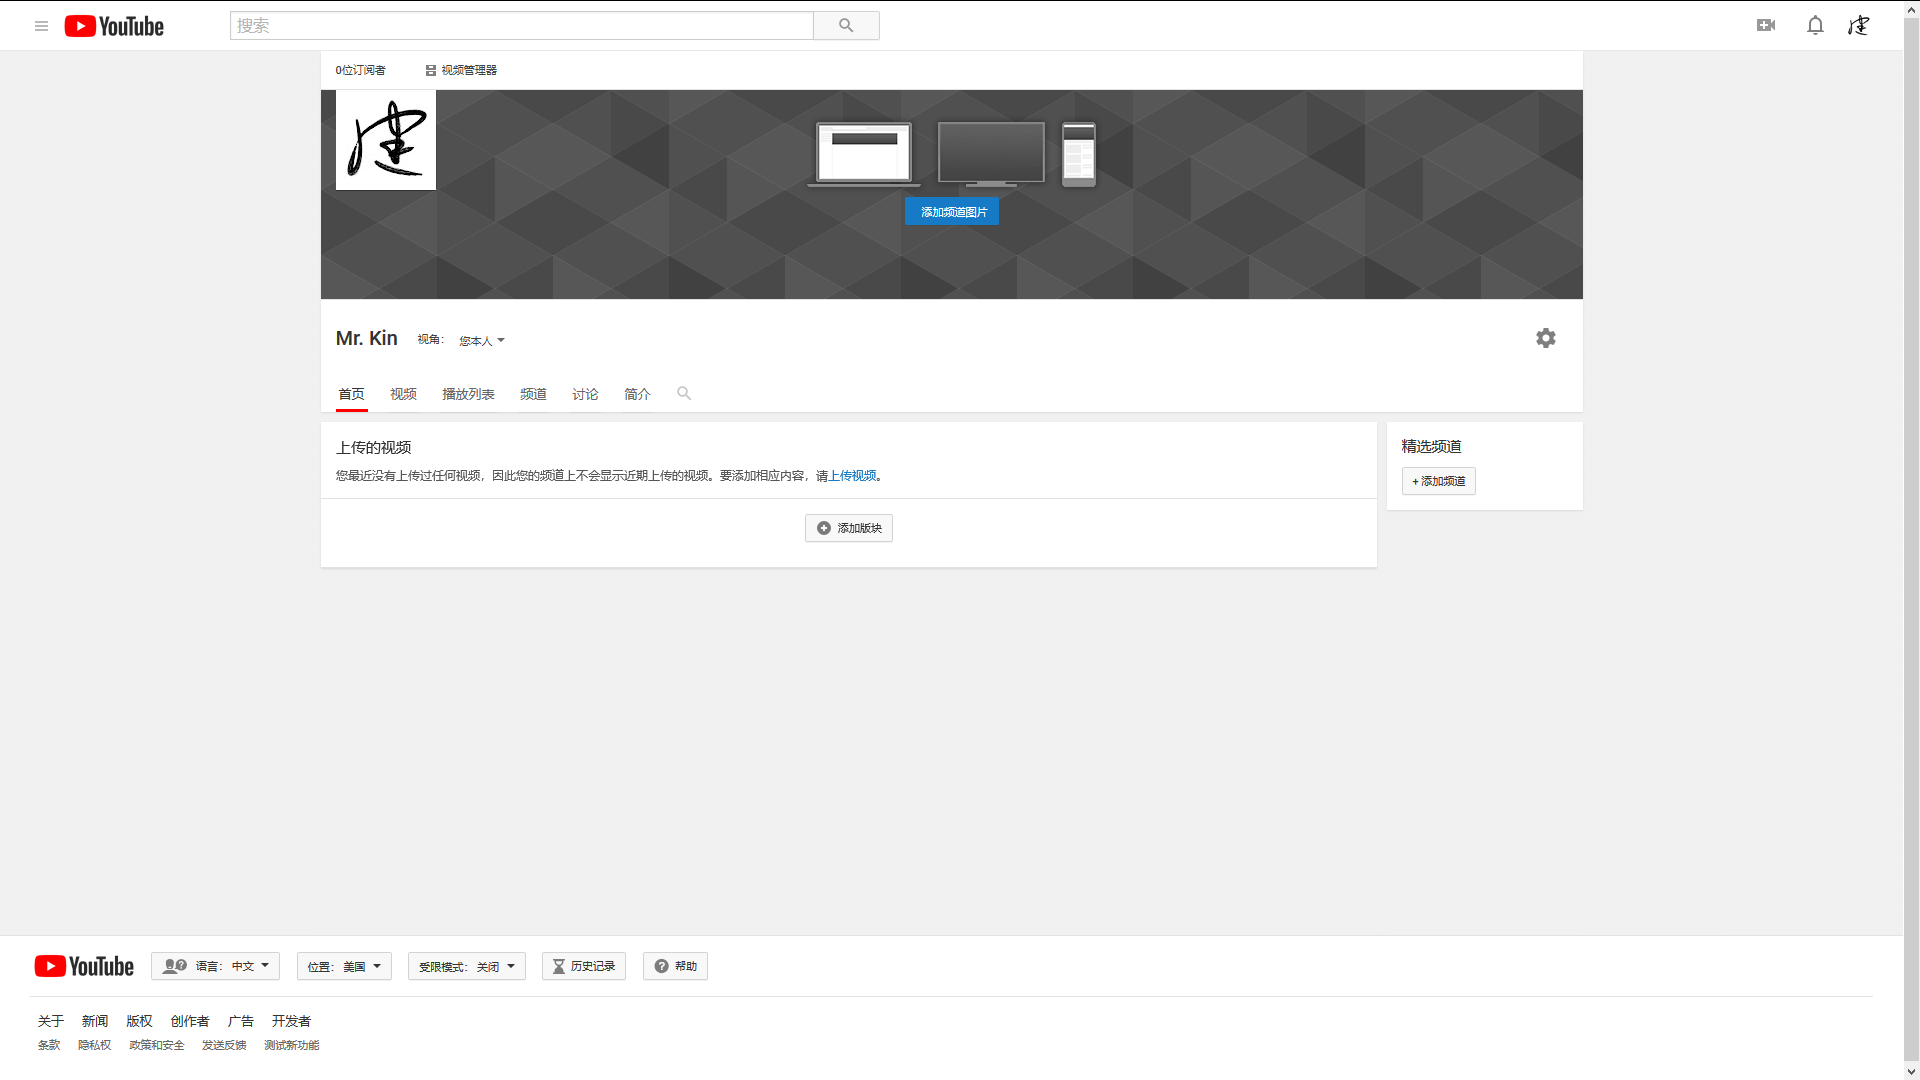
\includegraphics[scale=0.055]{Youtube}
    \end{minipage}
\end{figure}
 % 出于特殊的安全设置,\include 命令无法使用相对路径,因为需要读写权限以给 included file 写 aux 文件,而 \input 命令只需要读权限。
    \clearpage
    \phantomsection
\begin{center}
    {\bfseries\sffamily\Large 版权声明}
\end{center}
\addcontentsline{toc}{chapter}{版权声明}

\noindent 作者:Mr. Kin \\
\DetectToksEmpty\LinkBlogPost
\ifToksEmpty
博文链接:链接暂空\\
\else
博文链接:\href{\the\LinkBlogPost}{跳转博文页}\\
\fi
\DetectToksEmpty\LinkPDFSource
\ifToksEmpty
PDF及LaTex源码链接:链接暂空\\
\else
PDF及LaTex源码链接:\href{\the\LinkPDFSource}{跳转PDF及LaTex源码页}\\
\fi
\DetectToksEmpty\LinkVideo
\ifToksEmpty
\else
相关视频创作链接:\href{\the\LinkVideo}{跳转视频页}\\
\fi
许可协议:本作品的所有内容,除个人设计创作的图像(如logo等)和相关的视频创作及其他特别声明外,均采用\href{https://creativecommons.org/licenses/by-nc-sa/4.0/deed.zh}{知识共享\ 署名-非商业性使用-相同方式共享 4.0 国际许可协议}进行发布。版权 © Mr. Kin,保留所有权利。
\includegraphics[scale=.4]{CC-BY-NC-SA}\\*[1.3ex]
\begin{tabular}{|*{3}{p{0.306\textwidth}|}}
    \hline
    \textsf{\bfseries 允许} & \textsf{\bfseries 限制} & \textsf{\bfseries 条件} \\
    \hline
    \vspace{-8pt}{\color{green}√} 修改 & \vspace{-8pt}{\color{red}×} 商标使用 & \vspace{-8pt}{\color{blue}$\odot$} 保留原署名 \\[-12pt]
    {\color{green}√} 分发 & {\color{red}×} 专利使用 & {\color{blue}$\odot$} 状态变更说明 \\[-12pt]
    {\color{green}√} 个人使用 & {\color{red}×} 商业使用 & {\color{blue}$\odot$} 相同的许可和版权声明 \\
    \hline
\end{tabular}
\\*[1.3ex]
\emph{注:若想对本作品进行转载、引用亦或是进行二次创作时,请详细阅读上述相关协议内容(若不理解,请点击链接跳转阅读)。为保障本人权利,对于违反者,本人将依法予以处理!望周知!——Mr. Kin}

\begin{center}
    {\bfseries\sffamily\Large 勘误声明}
\end{center}

虽本人写作时已尽力保证其内容的正确性,但因个人知识面和经验的局限性以及计算机技术等相关技术日新月异,本作品内容或存在一些错误之处。还望诸君发现错误后能够\hyperlink{contact}{联系我}以更正错误,不胜感激!——Mr. Kin

\begin{center}
    {\bfseries\sffamily\Large 侵权声明}
\end{center}

若本作品采用的第三方内容侵犯了你的版权,请与我\hyperlink{contact}{联系}进行处理,谢谢!——Mr. Kin

\begin{center}
    {\bfseries\sffamily\Large 第三方开源许可声明}
\end{center}

\noindent 本作品使用的第三方开源产品有:
\begin{multicols}{2}
\begin{itemize}
    \item \href{https://github.com/adobe-fonts}{Adobe Fonts}: \href{https://github.com/adobe-fonts/source-serif-pro/blob/release/LICENSE.md}{OFL v1.1}
    \item \href{https://tug.org/texlive/}{Tex Live}: \href{https://tug.org/texlive/copying.html}{TeX Live Licensing}
    \item \href{https://code.visualstudio.com/}{Visual Studio Code}: \href{https://github.com/Microsoft/vscode/blob/master/LICENSE.txt}{MIT}
    \item \href{http://ffmpeg.org/}{FFmpeg}: \href{http://ffmpeg.org/legal.html}{LGPL v2.1 / GPL v2}
    \item \href{https://krita.org/en/}{Krita}: \href{https://docs.krita.org/en/KritaFAQ.html?highlight=license#license-rights-and-the-krita-foundation}{Krita's GPL license}
    \item \href{https://inkscape.org/}{Inkscape}: \href{https://inkscape.org/about/license/}{GPL}
    \item \href{https://www.gimp.org}{GIMP}: \href{https://www.gimp.org/about/COPYING}{GPL}
    \item \href{https://www.blender.org}{Blender}: \href{https://www.blender.org/about/license/}{GPL}
    \item \href{https://www.audacityteam.org/}{Audacity}: \href{https://www.audacityteam.org/about/license/}{GPL v2}
    \item \href{https://handbrake.fr}{Handbrake}: \href{https://github.com/HandBrake/HandBrake/blob/master/LICENSE}{GPL v2}
\end{itemize}
\end{multicols}

\noindent 更多请点击查看\href{https://mister-kin.github.io/about/third-party-declaration/}{第三方声明页}!

    \clearpage
    {\centering \tableofcontents} % 生成目录页。
    \mainmatter

    % 正文
    \chapter{切换语言}
    \section{介绍}
    一款blender插件,旨在通过一键快速、轻松地在两种语言之间切换用户界面,而非重复打开偏好设置。

    \subsection{背景}
    在早期进行blender手册翻译工作时,因需要校对相关UI内容,本人频繁地在中英文之间切换软件的用户界面语言。但每次繁琐地使用偏好设置进行语言切换令人苦不堪言,索性就开发一款插件以简化这操作。

    \subsection{面向人群}
    \begin{itemize}
        \item 翻译者:需要频繁切换界面语言以校对相关内容。
        \item CG学习者:需要频繁切换界面语言才能跟进外语教程。
    \end{itemize}

    \subsection{插件目前实现的功能}
    \begin{itemize}
        \item 一键切换UI语言(目前仅支持:简中/英)
        \item 一键打开用户偏好设置
        \item 插件的个性化设置菜单
        \item 一键设置自定义的「用户偏好设置」({\color{red}该功能还处于试验性中,慎用})
    \end{itemize}
    \noindent {\footnotesize \emph{注:更多详细介绍请查看「\hyperlink{AddonFeatures}{插件功能}」小节内容,规划中的功能请\href{https://mister-kin.github.io/roadmap/}{跳转蓝图规划页}查看。}}

    \section{用法}

    \subsection{下载及安装}
    \noindent {\bfseries \sffamily 下载步骤}\par
    \begin{itemize}
        \item 下载地址:\href{https://github.com/Mister-Kin/ToggleLanguage/releases/latest}{点击跳转},下载ToggleLanguage.zip文件。
        \item blender版本要求:\href{https://www.blender.org/download/}{v2.83+}
    \end{itemize}

    \noindent {\bfseries \sffamily 安装步骤}
    \begin{enumerate}
        \item 打开「Preferences/用户偏好设置」(Menu/菜单>Edit/编辑>Preferences/用户偏好设置)。
        \item 选择「Add-ons/插件」选项卡。
        \item 点击「Install.../安装」后,选择先前所下载好的ToggleLanguage.zip并点击确定。
        \item 启用插件。
    \end{enumerate}

    \begin{figure}[htbp]
        \begin{minipage}[t]{0.45\textwidth}
            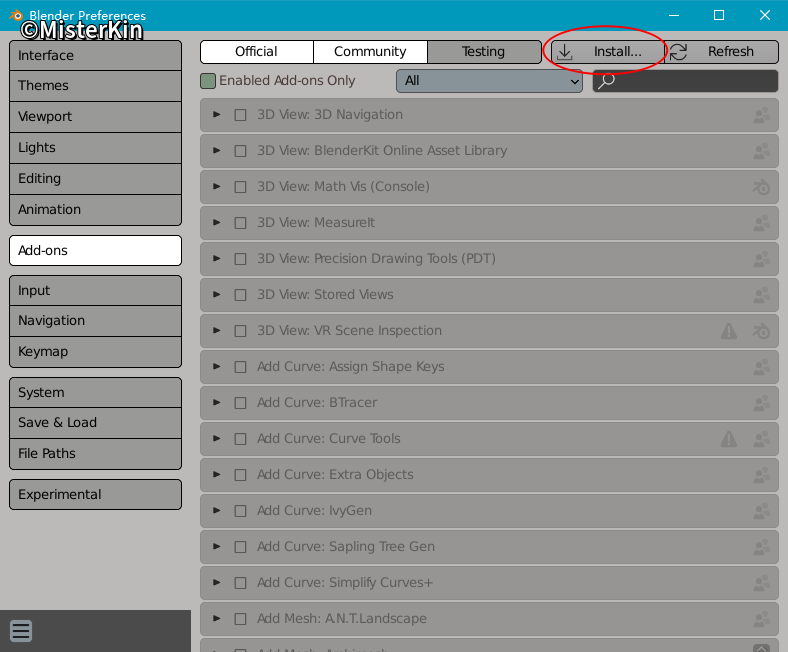
\includegraphics[scale=0.26]{Installation}
            \caption{安装方法}
        \end{minipage}
        \qquad
        \begin{minipage}[t]{0.45\textwidth}
            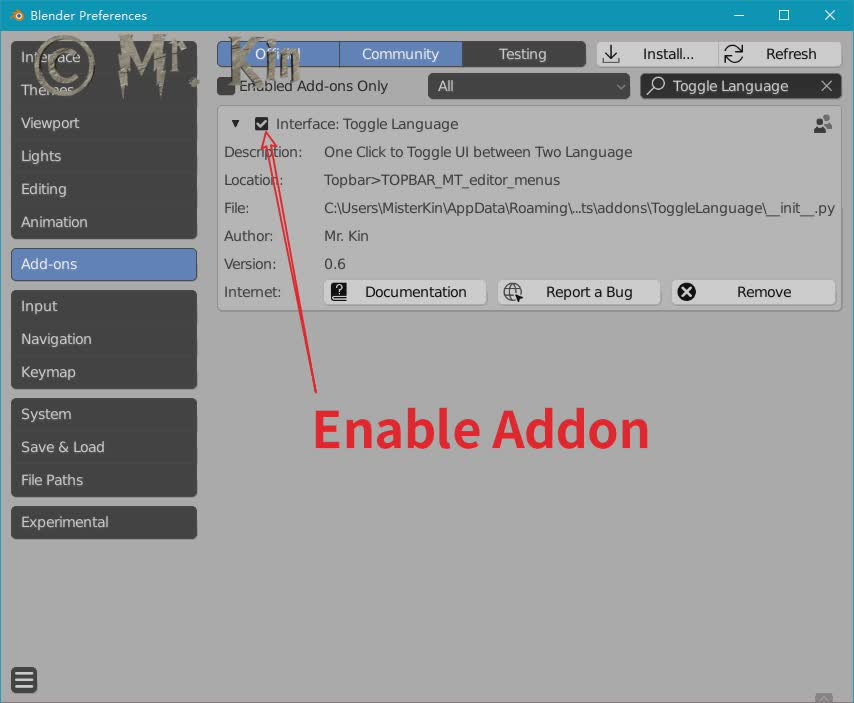
\includegraphics[scale=0.26]{EnableAddon}
            \caption{启用插件}
        \end{minipage}
    \end{figure}

    \subsection{插件UI}
    \label{插件UI小节}
    \begin{figure}[htbp]
        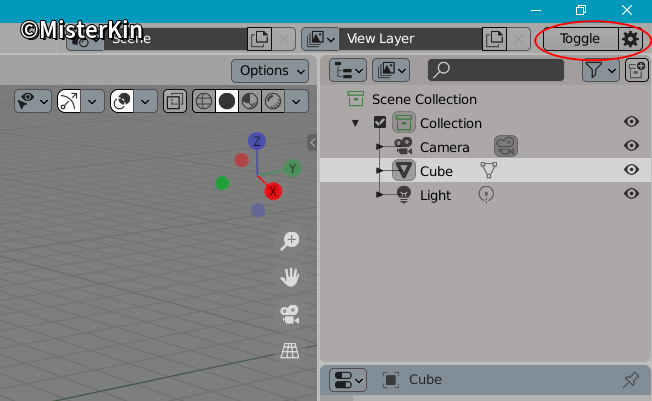
\includegraphics[scale=0.24]{UI}
        \caption{插件UI(图示菜单已被下拉展开)}\label{插件UI}
    \end{figure}

    如图\ref{插件UI}所示,启用插件后,可看见插件位于顶端菜单栏末尾处。插件UI从左往右看,有三个元素:
    \begin{enumerate}
        \item 左侧是语言切换按钮。
        \item 中间是插件的个性化设置菜单。
        \item 右侧是用户偏好设置按钮。
    \end{enumerate}

    \subsection{插件功能}
    \hypertarget{AddonFeatures}{}
    \noindent {\footnotesize \em 注:以下按照UI排布位置进行功能介绍。UI排布位置详见\ref{插件UI小节}小节。}
    \begin{enumerate}
        \item 语言切换按钮(快捷键F5):切换blender用户界面语言(目前仅支持:简中/英)。
        \item 设置菜单:插件的个性化设置。
        \begin{enumerate}
            \item UI提示方案菜单:选择相应UI提示的方案。
            \begin{enumerate}
                \item 默认模式:关闭「开发选项」「Python工具提示」,如图\ref{UI提示方案菜单:默认模式}所示。
                \item 开发者模式:启用「开发选项」「Python工具提示」,如图\ref{UI提示方案菜单:开发者模式}所示。
            \end{enumerate}
            \item 新建数据-翻译按钮:启用/关闭新建数据的翻译功能,默认值为关闭,如图\ref{新建数据选项}所示。在非英语界面环境中,启用该功能可使blender新建数据的名称为当前语言,如图\ref{新建数据效果}所示,新建平面的名称为「平面」,而非「plane」。
            \item 我的偏好设置按钮({\color{red}试验性,慎用}):部署我个人的偏好设置。所涉及的设置选项详见\hyperlink{MyPreferences}{我的偏好设置}。(注意:使用该功能,同时会将一些设置保存进启动文件中。然而重置偏好设置按钮无法重置启动文件,\marginpar{\scriptsize 在测试中,使用插件来重置启动文件会导致blender闪退,故只保留重置偏好设置的功能。}如果需要还原所有设置,除了使用插件的重置按钮,仍需使用「Menu/菜单>File/文件>Default/默认>Load Factory Settings/加载初始设置」以重置启动文件。)
            \item 重置偏好设置按钮:重置偏好设置。
        \end{enumerate}
        \item 用户偏好设置按钮(快捷键Ctrl+Alt+U):打开用户偏好设置窗口。
        \item PS:搜索功能增设快捷键F6(因本人有其他软件占用全局快捷键F3,故增设F6键)
    \end{enumerate}

    \begin{figure}[htbp]
        \begin{minipage}[t]{0.45\textwidth}
            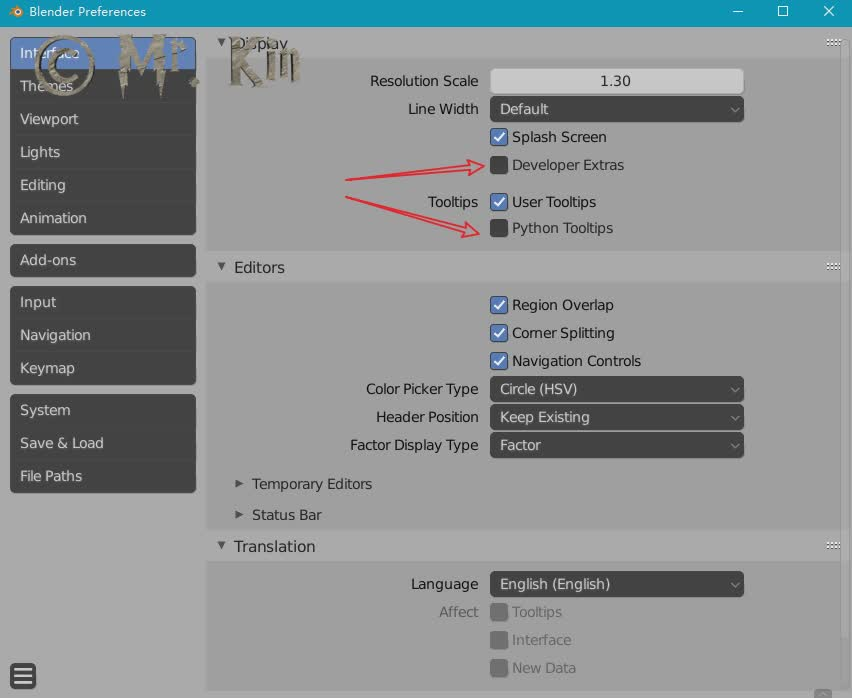
\includegraphics[scale=0.26]{DefaultHint}
            \caption{UI提示方案菜单:默认模式}
            \label{UI提示方案菜单:默认模式}
        \end{minipage}
        \qquad
        \begin{minipage}[t]{0.45\textwidth}
            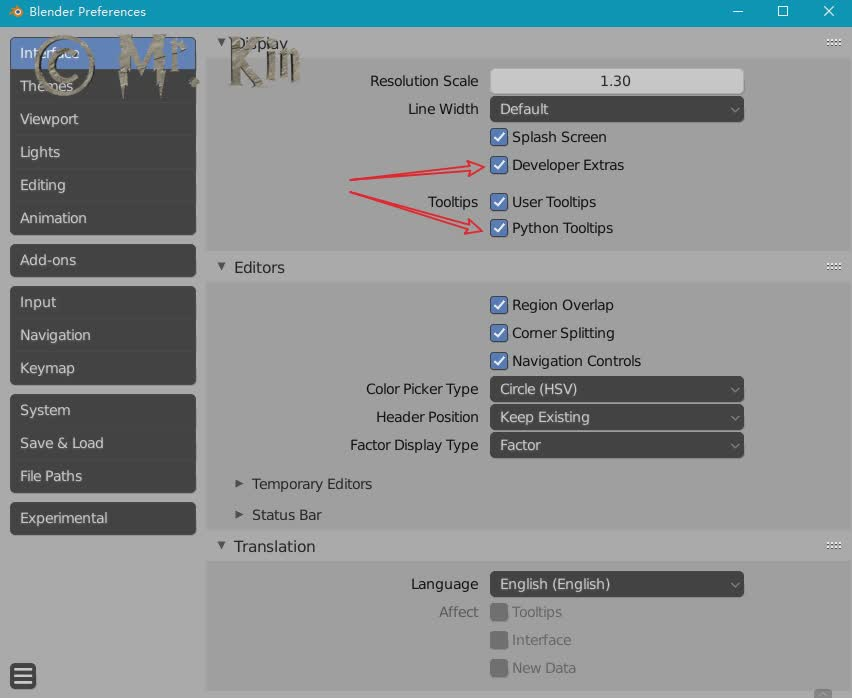
\includegraphics[scale=0.26]{DeveloperHint}
            \caption{UI提示方案菜单:开发者模式}
            \label{UI提示方案菜单:开发者模式}
        \end{minipage}

        \vspace{1ex}

        \begin{minipage}[t]{0.38\textwidth}
            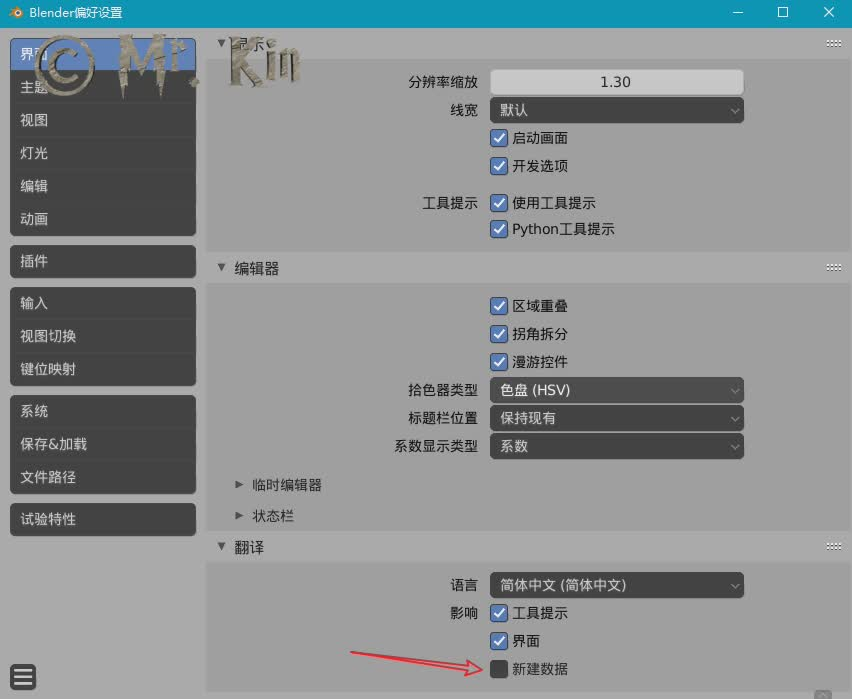
\includegraphics[scale=0.20]{NewDataOption}
            \caption{新建数据-翻译按钮启用/关闭的选项}
            \label{新建数据选项}
        \end{minipage}
        \begin{minipage}[t]{0.65\textwidth}
            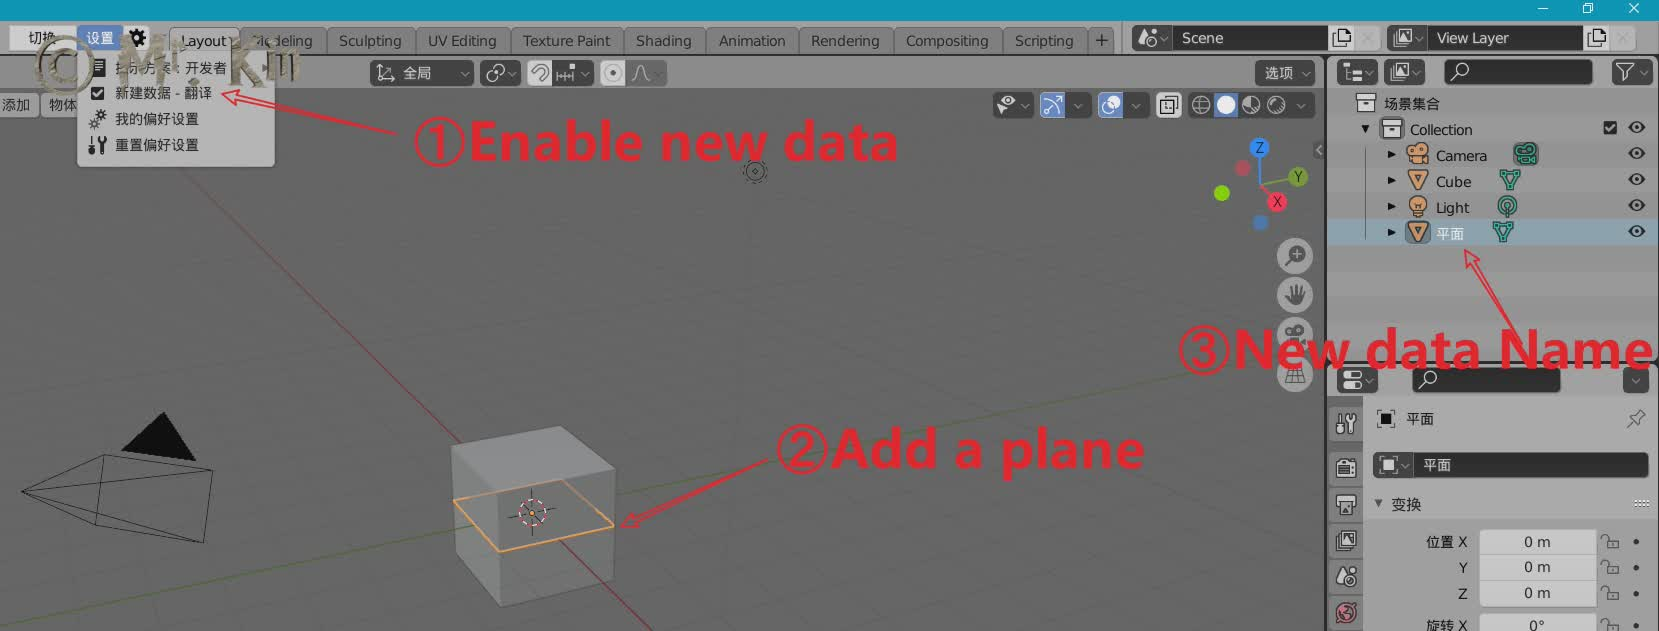
\includegraphics[scale=0.18]{NewDataEffect}
            \caption{新建数据-翻译按钮启用后的效果:图示界面语言为中文}
            \label{新建数据效果}
        \end{minipage}
    \end{figure}

    \newpage
    \noindent {\bfseries \sffamily \hypertarget{MyPreferences}{我的偏好设置}(我本人的一些设置习惯)}\par
    \begin{enumerate}
        \item 偏好设置部分:
        \begin{enumerate}
            \item 界面>分辨率缩放到1.3
            \item 主题>Blender Light
            \item 插件>启用插件Node Wrangler、Cell Fracture、Auto Tile Size、Development: Icon Viewer。
            \item 视图切换>启用「围绕选择物体选择」和「缩放至鼠标位置」。
            \item 键位映射>启用「Pie Menu on Drag」和「Extra Shading Pie Menu Items」。
            \item 系统
            \begin{enumerate}
                \item Cycles渲染设备>CUDA
                \item 声音>音频设备>SDL
            \end{enumerate}
            \item 报错\&加载>启用「压缩文件」、关闭「自动保存」
            \item 文件路径
            \begin{enumerate}
                \item 纹理:H:\textbackslash Textures\textbackslash
                \item 临时文件:E:\textbackslash Temp\textbackslash
                \item 渲染输出:E:\textbackslash Process\textbackslash
                \item 渲染缓存:E:\textbackslash Temp\textbackslash
            \end{enumerate}
        \end{enumerate}
        \item 启动界面部分(注意:使用「我的偏好设置」功能,会同时将以下设置保存进启动界面文件):
        \begin{enumerate}
            \item 属性编辑器
            \begin{enumerate}
                \item 渲染属性
                \begin{enumerate}
                    \item 渲染引擎>Cycles
                    \item 设备>GPU计算
                    \item 采样>启用「自适应采样」
                    \item 性能>Auto Tile Size>Target Tile Size>256
                    \item 性能>线程>多线程模式>固定
                    \item 性能>线程>线程>6
                \end{enumerate}
                \item 输出属性>输出路径:E:\textbackslash Process\textbackslash
            \end{enumerate}
        \end{enumerate}
        \item 状态栏>启用「场景统计数据」「系统内存」「显存」
    \end{enumerate}

    \section{开发记录}
    \subsection{开发测试环境}
    \begin{itemize}
        \item Win10 v20H2 OS
        \item Blender v2.92
    \end{itemize}

    \noindent {\footnotesize \emph{注:建议在 blender v2.83 以上使用。2.83默认是启用翻译功能,2.83以下版本的翻译都得手动启用。因为没有实际测试过,所以2.83以下版本要使用该插件,可能需要手动启用翻译功能。这也是我将插件最低支持版本改为2.83的原因,当然,你也可在2.83以下的版本使用。}

    \newpage
    \subsection{更新历史}
    \begin{table}[!h]
        \centering
    \begin{tabular}{|*{2}{c|}p{240pt}|c|}
        \hline
        版本 & 更新日期 & \centering{更新内容} & 标签 \\
        \hline
        v0.6 & 2021/3/10 & 添加布尔值按钮-新数据翻译;支持快捷键;代码重构,插件翻译重构…… & Features \\
        \hline
        v0.5 & 2020/12/8 & 支持Blender v2.91;支持从.zip文件安装插件…… & Changes \\
        \hline
        v0.5-beta & 2020/9/20 & 添加菜单用以选择UI提示方案 & Features\\
        \hline
        v0.4 & 2020/8/3 & 代码项目重命名为ToggleLanguage;按钮UI放置于最右端;添加新按钮以快速查看preferences & Features \\
        \hline
        v0.3 & 2020/6/5 & 更新至blender 2.83 api;修改部分类名;添加文档链接;修改完善许可说明 & Minor changes \\
        \hline
        v0.2 & 2020/5/21 & 清除未使用属性的报错 & Bug fixes \\
        \hline
        v0.1 & 2020/5/12 & 完成基础的功能设计「一键切换」 & Features \\
        \hline
    \end{tabular}
    \end{table}

    \noindent {\footnotesize \em 注:更多详细的信息,请查看\href{https://github.com/Mister-Kin/ToggleLanguage/releases}{Release Notes}。}

    \section{作者}
    \textbf{ToggleLanguage} © Mr. Kin, 项目代码采用 \href{https://github.com/Mister-Kin/ToggleLanguage/blob/master/LICENSE}{GNU GPL v3.0} 许可协议进行发布。

    由 Mr. Kin 著作并维护。

    \nocite{*} % 不使用 cite 也能生成参考文献。
    \printbibliography % 生成参考文献排版。
    \addcontentsline{toc}{chapter}{参考文献} % 添加参考文献进目录。

    \appendix
    % 附录

\end{document}
